\documentclass{article}
\usepackage[utf8]{inputenc}
\usepackage{indentfirst}
\usepackage{titling}
\usepackage{geometry}
\usepackage{graphicx}
\graphicspath{ {./Images/} }
\usepackage[shortlabels]{enumitem}
\usepackage{fancyhdr}
\usepackage{ulem}
\usepackage[dvipsnames]{xcolor}
\usepackage{amssymb}
\usepackage{listings}
\usepackage{color}

\definecolor{dkgreen}{rgb}{0,0.6,0}
\definecolor{gray}{rgb}{0.5,0.5,0.5}
\definecolor{mauve}{rgb}{0.58,0,0.82}

\lstset{frame=tb,
  language=Java,
  aboveskip=3mm,
  belowskip=3mm,
  showstringspaces=false,
  columns=flexible,
  basicstyle={\small\ttfamily},
  numbers=none,
  numberstyle=\tiny\color{gray},
  keywordstyle=\color{blue},
  commentstyle=\color{dkgreen},
  stringstyle=\color{mauve},
  breaklines=true,
  breakatwhitespace=true,
  tabsize=3
}

\def\ojoin{\setbox0=\hbox{$\bowtie$}%
  \rule[-.02ex]{.25em}{.4pt}\llap{\rule[\ht0]{.25em}{.4pt}}}
\def\leftouterjoin{\mathbin{\ojoin\mkern-5.8mu\bowtie}}
\def\rightouterjoin{\mathbin{\bowtie\mkern-5.8mu\ojoin}}
\def\fullouterjoin{\mathbin{\ojoin\mkern-5.8mu\bowtie\mkern-5.8mu\ojoin}}

\renewcommand\maketitlehooka{\null\mbox{}\vfill} %para centralizar verticalmente
\renewcommand\maketitlehookd{\vfill\null}
\pagestyle{fancy}
\fancyhf{}
\rfoot{\thepage}
\lfoot{ 
\includegraphics[scale=0.01]{UA.jpg} José Mendes 107188 LEI}
\geometry{
  a4paper,
  headheight=4cm,
  top=5.5cm,
  bottom=4.5cm,
  footskip=4cm
}


\title{Segurança Informática e nas Organizações - Resumos 2}
\author{José Mendes 107188}
\date{2023/2024}

\begin{document}


\begin{titlepage}
    \maketitle
    \begin{center}
        
\includegraphics[scale=0.4]{UA.png}
    \end{center}
    \thispagestyle{empty} %remove o count da pagina
\end{titlepage}

\pagebreak

\section{Criptografia Assimétrica}

\subsection{Criptografia Assimétrica (de blocos)}

\begin{flushleft}
  \textbf{Usa um par de chaves:}
  \begin{itemize}
    \item \textbf{Chave privada:} pessoal, não transmissível;
    \item \textbf{Chave pública:} disponível a todos;
  \end{itemize}

  \vspace{2mm}

  \textbf{Permite:}
  \begin{itemize}
    \item Confidencialidade sem qualquer exchange of secrets prévia;
    \item Autenticação
    \begin{itemize}
      \item De conteúdos (integridade dos dados);
      \item De origem (atenticação da source, ou assinatura digital);
    \end{itemize}
  \end{itemize}
\end{flushleft}

\subsection{Operaçõees de uma Cifra Assimétrica}

\begin{center}
  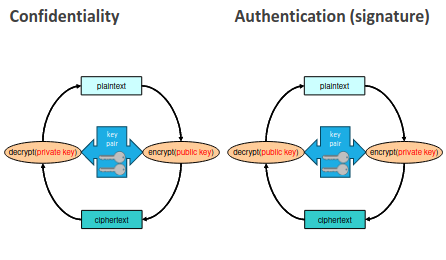
\includegraphics[scale=0.6]{1}
\end{center}

\subsection{Use Cases: Comunicação Segura}

\begin{flushleft}
  \textbf{Comunicação segura com um target (Bob)}
  \begin{itemize}
    \item A Alice encrípta o plaintext \textbf{P} com a chave pública do Bob, \textbf{Kpub\_Bob}
    \begin{itemize}
      \item \textbf{Alice: $C = \{P\}_{kpub\_bob}$}
    \end{itemize}
    \item O Bob decifra o ciphertext \textbf{C} com a sua chave privada, \textbf{Kpriv\_Bob}
    \begin{itemize}
      \item \textbf{Bob: $P' = \{C\}_{kpriv\_bob}$}
    \end{itemize}
    \item $P'$ deve ser igual a \textbf{P} (é necessário verificar)
    \item \textbf{Kpub\_Bob} precisa de ser conhecida pela Alice
  \end{itemize}
\end{flushleft}

\pagebreak

\begin{center}
  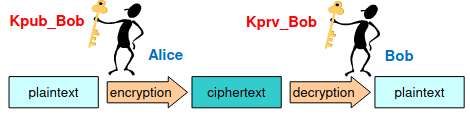
\includegraphics[scale=0.6]{2}
\end{center}

\subsection{Cifras Assimétricas}

\begin{flushleft}
  \textbf{Vantagens:}
  \begin{itemize}
    \item São um mecânismo de autenticação fundamental;
    \item Permitem explorar caracteristicas que não são possíveis com cifras simétricas;
  \end{itemize}

  \vspace{2mm}

  \textbf{Desvantagens:}
  \begin{itemize}
    \item Performance;
    \item Normalmente não são muito eficientes e consomem muita memória;
  \end{itemize}

  \vspace{2mm}
  \textbf{Problemas:}
  \begin{itemize}
    \item Distribuição confiável de chaves públicas;
    \item O lifetime do par de chaves é limitado;
  \end{itemize}

  \vspace{2mm}

  \textbf{Abordagens: problemas matemáticos complexos}
  \begin{itemize}
    \item Logaritmos discretos de números grandes;
    \item Factorização inteira de números grandes;
  \end{itemize}

  \vspace{2mm}
  \textbf{Algoritmos mais comuns:}
  \begin{itemize}
    \item RSA;
    \item ElGamal;
    \item Eliptic Curves (ECC);
  \end{itemize}

  \vspace{2mm}

  \textbf{Outras tecnicas com pares assimétricos de chaves:}
  \begin{itemize}
    \item Diffie-Hellman (key agreement);
  \end{itemize}
\end{flushleft}

\pagebreak

\subsection{RSA (Rivest, Shamir, Adelman, 1978)}

\begin{flushleft}
  \textbf{Chaves:}
  \begin{itemize}
    \item \textbf{Privada:} (d, n)
    \item \textbf{Pública:} (e, n)
  \end{itemize}

  \vspace{2mm}

  \textbf{Encriptação da chave pública (confidencialidade)}
  \begin{itemize}
    \item $C = P^e \hspace{2mm} mod \hspace{2mm} n$
    \item $P = C^d \hspace{2mm} mod \hspace{2mm} n$
  \end{itemize}

  \vspace{2mm}

  \textbf{Encriptação da chave privada (assinatura)}
  \begin{itemize}
    \item $C = P^d \hspace{2mm} mod \hspace{2mm} n$
    \item $P = C^e \hspace{2mm} mod \hspace{2mm} n$
  \end{itemize}

  \begin{center}
    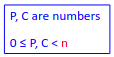
\includegraphics[scale=0.6]{3}
  \end{center}

  \textbf{Complexidade Computacional}
  \begin{itemize}
    \item Logaritmo discreto;
    \item Factorização inteira;
  \end{itemize}

  \vspace{2mm}

  \textbf{Seleção de Chaves}
  \begin{itemize}
    \item \textbf{n} grande (centenas ou milhares de bits);
    \item \textbf{$n = p \times q$} com \textbf{p} e \textbf{q} sendo números primos grandes (secretos);
    \item Escolher um \textbf{e} co-primo de \textbf{$(p-1) \times (q-1)$};
    \item Computar \textbf{d} tal que \textbf{$e \times d \equiv 1 \hspace{2mm} (mod \hspace{2mm} (p-1) \times (q-1))$};
    \item Discartar \textbf{p} e \textbf{q};
    \item O valor de \textbf{d} não pode ser facilmente computado a partir de \textbf{e} e \textbf{n} (apenas de \textbf{p} e \textbf{q});
  \end{itemize}
\end{flushleft}

\pagebreak

\subsubsection{RSA - Exemplo}

\begin{center}
  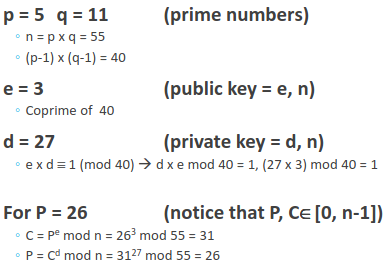
\includegraphics[scale=0.6]{4}
\end{center}

\subsection{Encriptação Hibrida}

\begin{flushleft}
  \textbf{Mistura criptografia simétrica com assimétrica}
  \begin{itemize}
    \item Usa o melhor dos dois mundos, evitando os problemas;
    \item Cifra assimétrica: usa chaves públicas (mas é lenta);
    \item Cifra simétrica: Rápida (mas com métodos fracos de troca de chaves);
  \end{itemize}

  \vspace{2mm}

  \textbf{Método}
  \begin{itemize}
    \item Obtém \textbf{$K_{pub}$} do destinatário;
    \item Gera uma chave simétrica aleatória \textbf{$K_{sym}$};
    \item Calcula \textbf{$C1 = E_{sym}(K_{sym}, P)$};
    \item Calcula \textbf{$C2 = E_{asym}(K_{pub}, K_{sym})$};
    \item Envia \textbf{$C1 + C2$};
    \begin{itemize}
      \item $C1$ é o texto encriptado com a chave simétrica;
      \item $C2$ é a chave simétrica encriptada com a chave pública do destinatário (pode também conter um IV);
    \end{itemize}
  \end{itemize}
\end{flushleft}

\subsection{Randomização de encriptações assimétricas}

\begin{flushleft}
  \textbf{Resultado de encriptações assimétricas não deterministico (não é prevísivel)}
  \begin{itemize}
    \item \textbf{N} encriptações do mesmo valor, com a mesma chave, deve produzir \textbf{N} resultados diferentes;
    \item \textbf{Objetivo:} Previnir a descoberta de valores encriptados através de tentativa e erro;
  \end{itemize}

  \vspace{2mm}

  \textbf{Abordagens:} Concatenação de um valor a encriptar com dois valores,
  um fixo (para controlo de integridade) e outro aleatório (para randomização);
\end{flushleft}

\subsubsection{OAEP (Optimal Asymmetric Encryption Padding)}

\begin{center}
  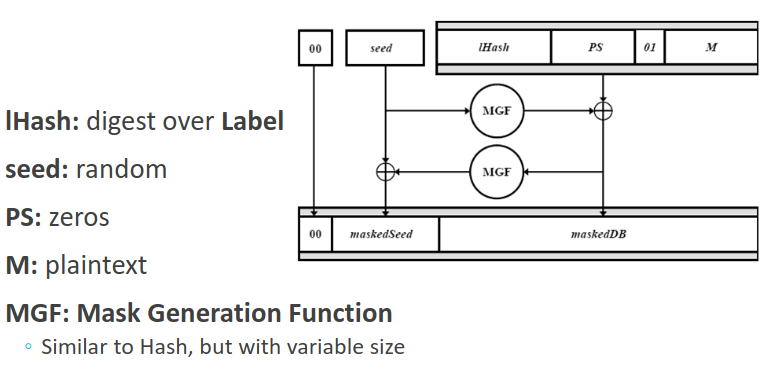
\includegraphics[scale=0.4]{5}
\end{center}

\subsection{Diffie-Hellman Key Agreement (1976)}

\begin{center}
  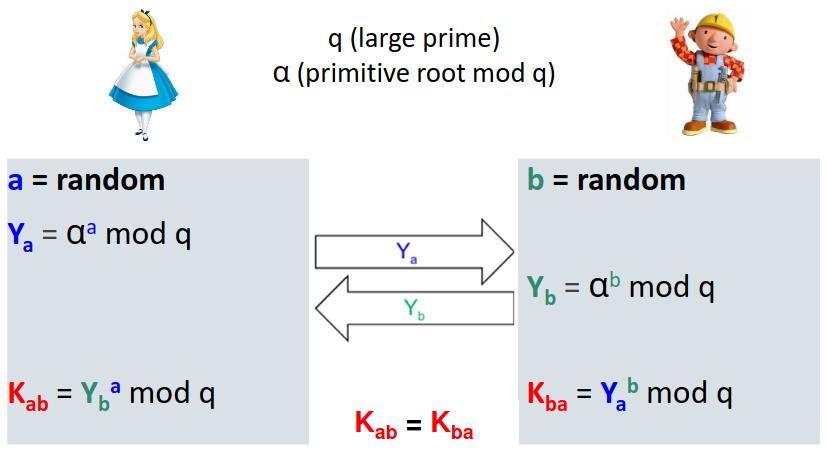
\includegraphics[scale=0.3]{6}
\end{center}

\subsubsection{DH Key Agreement: MitM Attack}

\begin{center}
  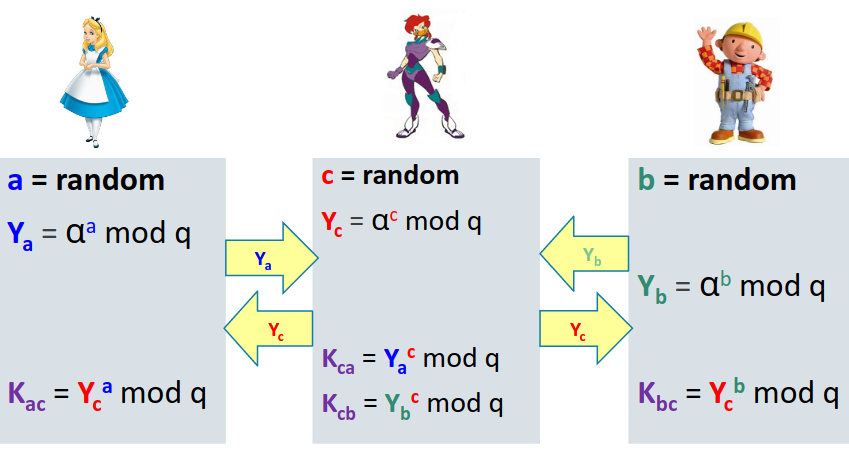
\includegraphics[scale=0.3]{7}
\end{center}

\pagebreak

\subsection{Eliptic Curve Cryptography (ECC)}

\begin{flushleft}
  \textbf{Curvas elipticas são funções específicas}
  \begin{itemize}
    \item Têm um gerador \textbf{G};
    \item Uma chave privada $K_{priv}$, é um inteiro com um máximo de
    bits permitidos pela curva;
    \item Uma chave pública $K_{pub}$, é um ponto $(x, y) = K_{priv} \times G$
    \item Dada $K_{pub}$, deve ser computacionalmente dificil determinar $K_{priv}$;
  \end{itemize}

  \begin{center}
    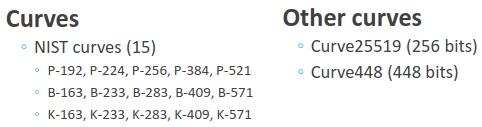
\includegraphics[scale=0.5]{9}
  \end{center}
\end{flushleft}

\subsection{ECDH: DH com ECC}

\begin{center}
  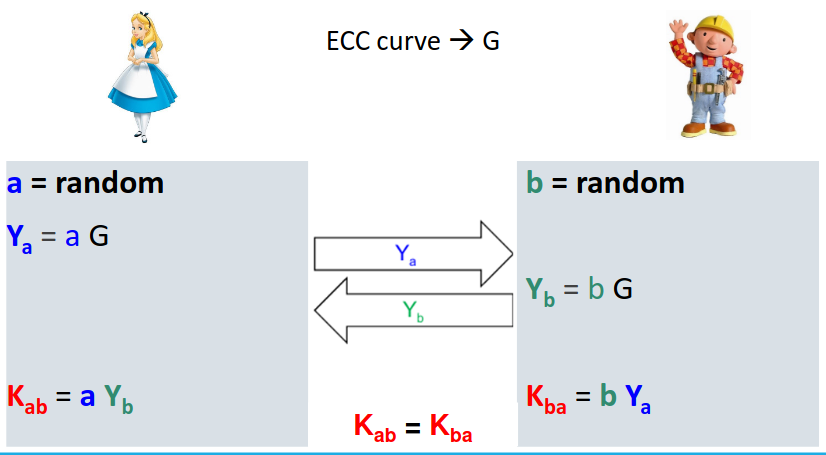
\includegraphics[scale=0.4]{8}
\end{center}

\subsection{Encriptação de chave pública com ECC}

\begin{flushleft}
  \textbf{Mistura encriptação hibrida com EDHC}

  \pagebreak

  \textbf{Método}
  \begin{itemize}
    \item Obtém $K_{pub\_recv}$ do destinatário;
    \item Gera um random $K_{priv\_send}$ com um correspondente $K_{pub\_send}$;
    \item Calcula $K_{sym} = K_{priv\_send} \times K_{pub\_recv}$;
    \item $C = E(P, K_{sym})$;
    \item Envia $C + K_{pub\_send}$;
    \vspace{2mm}
    \item Destinatário calcula $K_{sym} = K_{pub\_send} \times K_{priv\_recv}$;
    \item $P = D(C, K_{sym})$;
  \end{itemize}
\end{flushleft}

\section{Assinaturas digitais}

\subsection{Cifras Assimétricas (de blocos)}

\begin{flushleft}
  \textbf{Usa pares de chaves:}
  \begin{itemize}
    \item Uma \textbf{chave privada} (pessoal, não transmissível);
    \item Uma \textbf{chave pública} (disponível a todos);
  \end{itemize}

  \vspace{2mm}

  \textbf{Permite:}
  \begin{itemize}
    \item Confidencialidade sem qualquer exchange of secrets prévia;
    \item Autenticação
    \begin{itemize}
      \item De conteúdos (integridade dos dados);
      \item De origem (atenticação da source, ou assinatura digital);
    \end{itemize}
  \end{itemize}
\end{flushleft}

\subsection{Assinaturas Digitais}

\begin{center}
  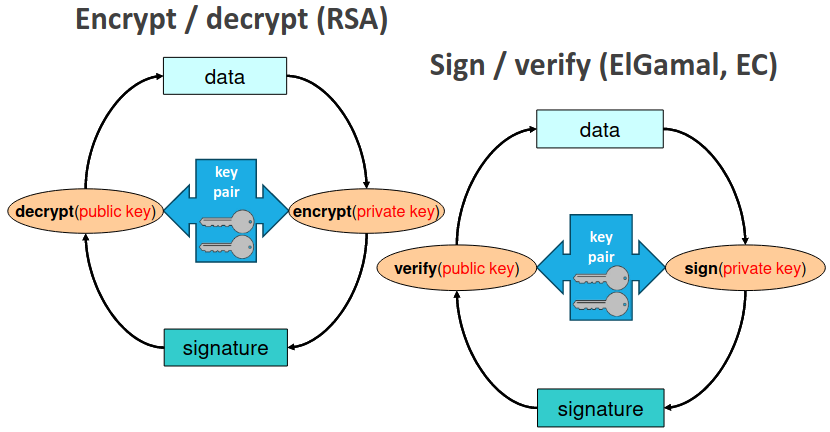
\includegraphics[scale=0.4]{10}
\end{center}

\pagebreak

\begin{flushleft}
  \textbf{Autenticação de conteúdos de um documento} - Garante a sua integridade
  (não se alterou);

  \vspace{2mm}

  \textbf{Autenticação do autor} - Garante que a identidade do criador/origem;

  \vspace{2mm}

  \textbf{Previnir repudiação de assinaturas}
  \begin{itemize}
    \item Non-repudiation (o autor não pode negar a autoria);
    \item Autores genuínos não podem negar a autoria (apenas a identidade
    do autor pode gerar uma dada assinatura);
  \end{itemize}

  \vspace{2mm}

  \textbf{Aboradgens}
  \begin{itemize}
    \item Encriptação/Decifração assimétrica ou assinatura/verificação;
    \item Funções digest (apenas para performance);
  \end{itemize}
\end{flushleft}

\begin{center}
  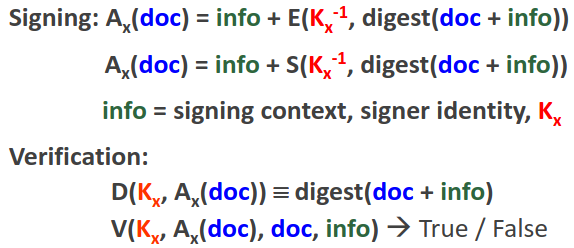
\includegraphics[scale=0.4]{11}
\end{center}

\subsubsection{Encriptação/Decifração signatures}

\begin{center}
  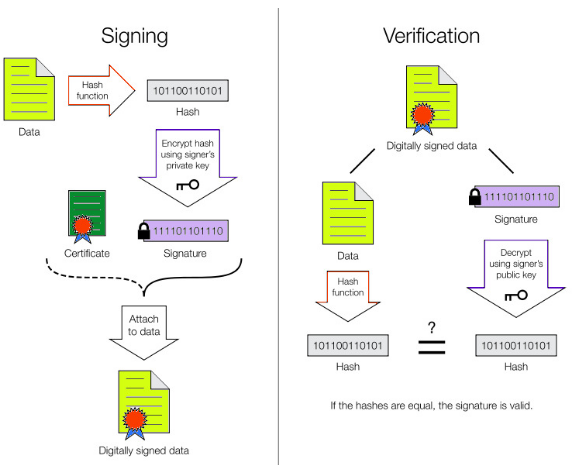
\includegraphics[scale=0.5]{12}
\end{center}

\pagebreak

\subsubsection{Assinatura digital num email: Multipart content, signature w/ certificate}

\begin{center}
  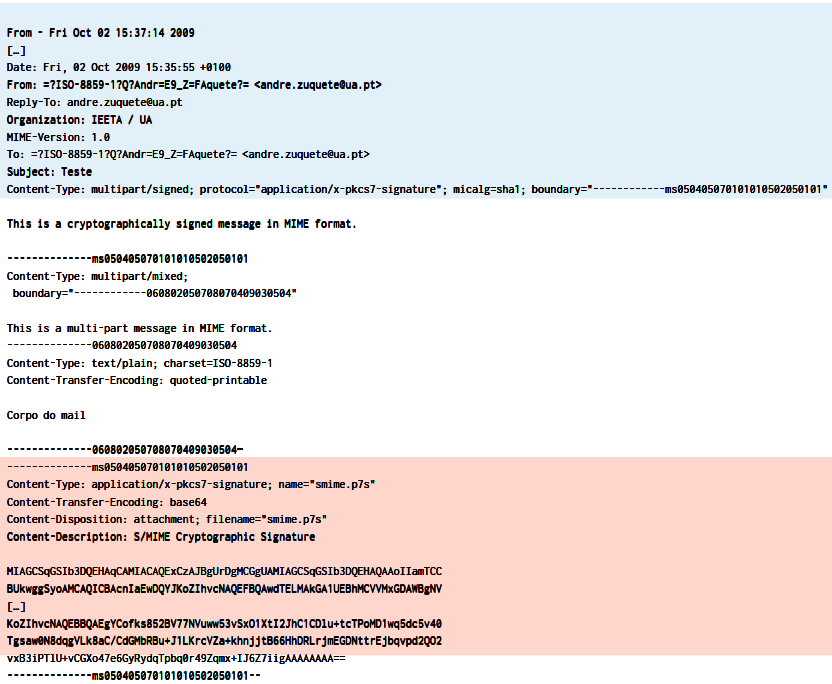
\includegraphics[scale=0.5]{13}
\end{center}

\pagebreak

\section{Derivação de chaves}

\begin{flushleft}
  \textbf{Algotitmos de cifras requerem chaves de tamanho fixo} - 56, 128, 256,\dots bits;

  \vspace{2mm}

  \textbf{Podemos derivar chaves de múltiplas origens}- shared secrets, passwords
  geradas por humanos, PIN codes e secrets de tamanho pequeno;

  \vspace{2mm}

  \textbf{Origem original pode ter baixa entropia} - reduz a dificuldade de
  ataques de força bruta, no entanto, devemos ter uma relação forte
  para uma chave útil;

  \vspace{2mm}

  \textbf{Por vezes percisamos de múltiplas chaves do mesmo material} -
  enquanto não permite encontrar o material (a password, outra chave)
  de uma chave nova;
\end{flushleft}

\subsection{Prepósitos de derivação de chaves}

\begin{flushleft}
  \textbf{Refroço de chaves: aumenta a segurança de uma password}
  \begin{itemize}
    \item Nomralmente definido por humanos;
    \item Tornando ataques de dicionário nada práticos;
  \end{itemize}

  \vspace{2mm}

  \textbf{Expansão de chaves: aumenta o tamanho de uma chave}
  \begin{itemize}
    \item Expande o tamanho que serve o algoritmo;
    \item Eventualmente deriva outras chaves relacionadas para outros algoritmos (ex: MAC);
  \end{itemize}
\end{flushleft}

\subsection{Derivação de chaves}

\begin{flushleft}
  \textbf{Derivação de chaves requer a existência de:}
  \begin{itemize}
    \item Um \textbf{salt} que trona a derivação única;
    \item Um problema difícil;
    \item Um nível de complexidade escolhido;
  \end{itemize}

  \vspace{2mm}

  \textbf{Dificuldade de Computação}
  \begin{itemize}
    \item A transformação requer recursos computacionais relevantes;
  \end{itemize}

  \vspace{2mm}

  \textbf{Dificuldade de Memória}
  \begin{itemize}
    \item A transformação requer recursos de armazenamento relevantes;
    \item Limita os ataques usando aceleração de hardware;
  \end{itemize}
\end{flushleft}

\pagebreak

\subsection{Derivação de chaves: PKBDF2}

\begin{flushleft}
  \textbf{Password Based Key Derivation Function 2}

  \vspace{2mm}

  \textbf{Produz uma chave a partir de uma password, com uma dificuldade escolhida}

  \[ K = PBKDF2(PRF, Salt, rounds, dim, password) \]

  \begin{itemize}
    \item \textbf{PRF} - Pseudo-Random-Function: função digest;
    \item \textbf{Salt} - Valor aleatório;
    \item \textbf{Rounds} - O custo computacional (dezenas ou centenas de milhares);
    \item \textbf{Dim} - Tamanho do resultado pretendido;
  \end{itemize}

  \vspace{2mm}

  \textbf{Operação: calcula operações ROUNDS x DIM a partir do PRF utilizando
  o SALT e a PASSWORD} - um tamanho maior de rounds aumenta a custo;
\end{flushleft}

\begin{center}
  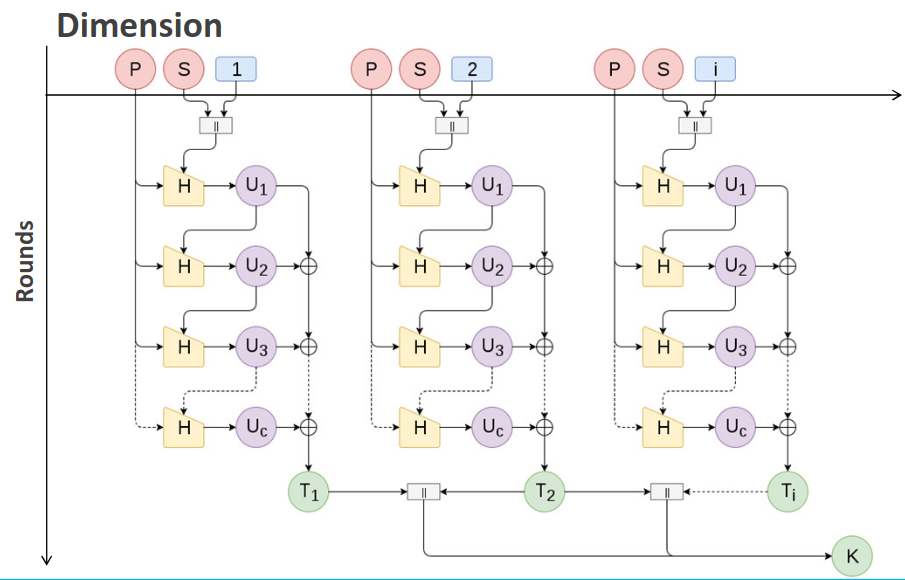
\includegraphics[scale=0.3]{14}
\end{center}

\pagebreak

\subsection{Derivação de chaves: Scrypt}

\begin{flushleft}
  \textbf{Produz uma chave com um custo de armazenamento escolhido}

  \vspace{2mm}

  \[ K = scrypt(password, salt, n, p, dim, r, hLen, Mflen) \]

  \begin{itemize}
    \item \textbf{Password} - Um segredo;
    \item \textbf{Salt} - Valor aleatório;
    \item \textbf{n} - Parâmetro de custo;
    \item \textbf{p} - Parâmetro de paralelismo $p \le (2^{32} -1) \times hLen / Mflen$;
    \item \textbf{dim} - Tamanho do resultado pretendido;
    \item \textbf{r} - Tamanho do bloco a usar (default: 8);
    \item \textbf{hLen} - Tamanho do da função digest (32 para SHA256);
    \item \textbf{Mflen} - Bytes na internal mix (default: $8 \times r$);
  \end{itemize}
\end{flushleft}

\begin{center}
  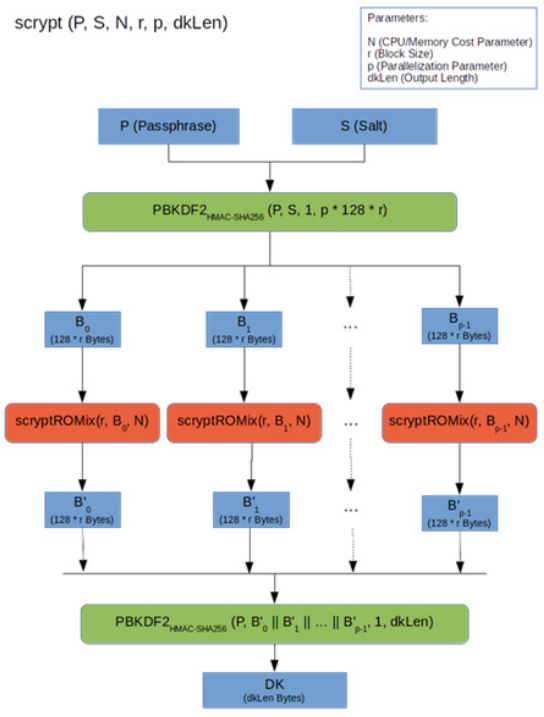
\includegraphics[scale=0.3]{15}
\end{center}

\pagebreak

\section{Gestão de chaves assimétricas}

\subsection{Problemas a resolver}

\begin{flushleft}
  \textbf{Garante um uso correto do par de chaves assimétricas}

  \begin{itemize}
     
  

    \item \textbf{Privacidade das chaves privadas}
    \begin{itemize}
      \item Garante a autenticidade;
      \item Previne a repudiação de assinaturas digitais;
    \end{itemize}

    \item \textbf{Distribuição correta de chaves públicas}
    \begin{itemize}
      \item Garante confidencialidade;
      \item Garante a correta validação de assinaturas digitais;
    \end{itemize}

  \end{itemize}

  \vspace{2mm}

  \textbf{Evolução temporal da entidade $\longleftrightarrow$ mapeamento de pares chave}

  \begin{itemize}
  
    \item \textbf{Para combater ocurrência catastróficas} (ex: perda de chaves privadas)

    \item \textbf{Para combater os requisitos de exploitations normais}
    (ex: refresh do par de chaves para reduzir riscos personificação)

  \end{itemize}

  \vspace{2mm}

  \textbf{Garante a correta geração de pares de chaves}
  \begin{itemize}
    \item \textbf{Geração aleatória de valores secretos}, de forma a poderem ser facilmente previstos;
    \item \textbf{Aumentar a eficiência sem reduzir a segurança}
    \begin{itemize}
      \item Tornar mecânismos de segurança mais eficientes;
      \item Aumentar a performance;
    \end{itemize}
  \end{itemize}
\end{flushleft}

\subsection{Objetivos}

\begin{flushleft}
  \begin{itemize}
    \item \textbf{Geração do par de chaves} - quando e como gerar;
    \item \textbf{Lidar com a chave privada} - como manter a chave privada;
    \item \textbf{Distribuição da chave pública} - como ditribuir corretamente as chaves públicas world-wide;
    \item \textbf{Tempo de vida do par de chaves} - quando vão expirar, até quando as usar e como verificar
    se esse par de chaves está obsuleto;
  \end{itemize}
\end{flushleft}

\pagebreak

\subsection{Geração de pares de chaves: Principais Designs}

\textbf{Usar bons geradores de números aleatórios para produzir segredos}

\begin{flushleft}
  \textbf{O resultado é indestinguível de noise}, isto é,
  todos os valores possíveis são igualmente prováveis e,
  não existem padrões resultantes do número da iteração ou de valores prévios;

  \vspace{2mm}

  \textbf{Exemplo: Bernoulli 1/2 Generator}
  \begin{itemize}
    \item Gerador sem memória;
    \item $P(b=1) = P(b=0) = 1/2$;
    \item Coin toss (atirar uma moeda ao ar);
  \end{itemize}
\end{flushleft}

\textbf{Facilidade sem comprometer a segurança}

\begin{flushleft}
  \textbf{Chaves públicas eficientes}
  \begin{itemize}
    \item Algumas são 1 bits, tipicamente $2k + 1$ valores (3, 17, 65537);
    \item Acelerar o processo com chaves públicas (o custo é proporcional ao número de bits 1);
    \item Sem security issues;
  \end{itemize}
\end{flushleft}

\textbf{Self-generation de chaves privadas}

\begin{flushleft}
  \textbf{Maximiza a privacidade, uma vez que outros nunca vão conseguir usar
  a dada chave privada}. Apenas o dono tem a chave, melhor ainda,
  o dono não tem a chave, mas pode usá-la;

  \vspace{2mm}

  \textbf{Principio pode ser relaxado quando não involve a geração de assinaturas}.
  Quando não existem issues relacionados com non-repudiation.
\end{flushleft}

\subsection{Lidar com chaves privadas}

\begin{itemize}
  \item \textbf{Correctness}
  
  \begin{itemize}
    \item \textbf{A chave privada representa o sujeito} (i.e., um cidadão, um servidor, etc.).
    O seu compromise deve ser minimizado. Cópias físicas seguras (backups) podem existir em alguns casos;

    \item \textbf{O caminho de acesso à chave privada deve ser controlado}.
    Proteção de acesso com password ou PIN code. Correctness das aplicações que usam;
  \end{itemize}

  \item \textbf{Confinement}
  \begin{itemize}
    \item \textbf{Proteção da chave privada dentro de um domínio seguro (reduzido) (ex: cryptographic token)}.
    O Token gera pares de chaves, exporta a chave pública mas nunca a privada, e, este Token
    encripta/decifra internamente com a chave privada.

    \item \textbf{Exemplo: SmartCards}, podemos pedir ao cartão para cifrar/decifrar
    algo. A chave privada nunca sai do SmartCard.
  \end{itemize}
\end{itemize}

\pagebreak

\subsection{Distribuição de chaves públicas}

\begin{flushleft}
  \textbf{Distribuição a todos os \uline{senders} de dados confidenciais}.
  Processo manual, usando um shared secret. Ad-hoc usando certificados digitais;

  \vspace{2mm}

  \textbf{Distribuição a todos os \uline{receivers} de assinaturas digitais}.
  Processo manual. Ad-hoc usando certificados digitais;
\end{flushleft}

\subsubsection{Problema}

\textbf{Como garantir a Correctness de uma chave pública?}

\vspace{2mm}

\textbf{Disseminação confiável de chaves públicas} - Paths/Graphs confiáveis.
Se \textbf{A confia em $K_X^+$} e \textbf{B confia em A}, então
\textbf{B confia em $K_X^+$}.

Hierarquias de certificação/grafos com as relações de confiança
expressas entre entidades. Certificação é unidirecional!

\subsection{Public key (digital) certificates}

É um \textbf{documento digital issued por uma autoridade de certificação (CA)}

\begin{itemize}
  \item \textbf{Liga a chave pública a uma entidade} (ex: pessoa, servidor ou serviço);
  \item \textbf{São documentos públicos}, não contêm informação privada,
  apenas pública. Pode ter informação adicional (ex: URL, nome, email, etc.);
  \item \textbf{São seguros criptograficamente},
  digitalmente assinados pelo issuer, não podem ser alterados;
\end{itemize}

\textbf{Pode ser usado para ditribuir chaves públicas de uma forma confiável}

\begin{flushleft}
  \textbf{O certificate receiver pode ser validade de várias formas}
  \begin{itemize}
    \item Com a chave pública do CA;
    \item Pode também validar a identificação;
    \item Validar a validade;
    \item Validar se a chave está a ser usada para o propósito correto;
  \end{itemize}

  \vspace{2mm}

  \textbf{O certificate receiver confia no comportamento do CA}, pelo que
  confia os documentos que este assina. Quando o CA associa um certificado a A,
  se o receicer confiar no CA, então confia que a associação de A é correta.
\end{flushleft}

\pagebreak

\begin{center}
  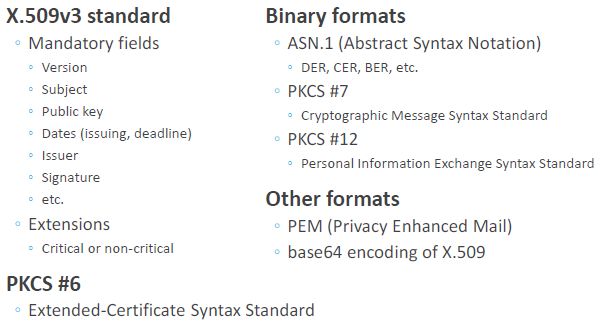
\includegraphics[scale=0.6]{16}
\end{center}

\subsection{Key pair usage}

\textbf{O certificado publico conecta o par de chaves a um perfil de utilização}.
As chaves privadas raramente são multifuncionais.

\vspace{2mm}

\textbf{Perfil de utilização tipico}
\begin{itemize}
  \item Autenticação/distribuição de chaves
  (Digital signature, Key encipherment, Data encipherment, Key agreement)
  \item Assinar documentos (Assinatura digital não repudiável)
  \item Certificate issuing (exclusivo de CAs). Assinar certificados,
  assinar CRLs (Certificate Revocation Lists)
  \item Timestamping (exclusivo de Time Stamping Authorities TSAs)
\end{itemize}

\textbf{Certificados de chaves públicas têm uma extensão para isto},
key usage (critical) que indica o perfil de utilização da chave pública.

\subsection{Assinatura de Certificados (CA)}

\begin{flushleft}
  \textbf{Organizações que gerem certificados de chaves públicas}.
  Companhias, não por lucro, governamentais, etc.;

  \vspace{2mm}

  \textbf{Define politicas e mecanismos para}:
  \begin{itemize}
    \item Issuing de certificados;
    \item Revoking de certificados;
    \item Distribuição de certificados;
    \item Issuing e distribuição das correspondentes chaves privadas;
  \end{itemize}

  \vspace{2mm}

  \textbf{Gerir a lista de certificados revogados} (CRLs), interfaces
  programaticas para verificar o estado atual de um certificado;
\end{flushleft}

\pagebreak

\subsection{Trusted Certification Authorities}

\begin{flushleft}
  \textbf{CAs intermediários} - CAs certificados por outras CAs confiaveis.
  Usando um certificado, permitindo a criação de uma hierarquia de certificação;

  \vspace{2mm}

  \textbf{Anchor confiavel (ou root CA)} - Um tem uma chave pública
  confiavel, normalmente implementada por certificados self-certified, ou seja,
  issuer e subject são o mesmo.

  Distribuição manual (ex: dentro do código do browser, OS, distribuição, etc.).
\end{flushleft}

Ver Exemplo de certificado nos slides 19-23.

\subsection{Refreshing of asymmetric key
pairs}

\begin{flushleft}
  \textbf{O par de chaves deve ter um tempo de vida limitado} - uma vez que,
  as chaves privadas podem ser perdidas ou descobertas, e para implementar
  uma politica de update;

  \vspace{2mm}

  \textbf{Problema} - Os certificados podem ser copiados e distribuidos.
  O universo de donos de certificados é desconhecido, pelo que, não podemos
  contactá-los para eliminar certificas específicos;

  \vspace{2mm}

  \textbf{Solução} - Certificados com um periodo de validade (nem antes, nem depois).
  Listas de certificados revogados, para revogar certificados
  antes da validade expirar;
\end{flushleft}

\subsection{Certificate Revocation Lists (CRLs)}

\begin{flushleft}
  \textbf{Base ou delta} - Completa / diferenças

  \vspace{2mm}

  \textbf{Listas de certificados assinados (identifiers) prematuramente
  invalidados} 
  \begin{itemize}
    \item Devem ser regularmente visitado por donos de certificados
    \item Protocolo OCSP para verificar a validade de um certificado (RFC 2560)
    \item Pode dizer a razão da revogação (slide 31)
  \end{itemize}

  \vspace{2mm}

  \textbf{Publicação e distribuição de CRLs} - Cada CA mantém
  a sua CRL e permite o acesso publico da mesma.
\end{flushleft}

\subsection{CRL e Delta CRL}

\begin{center}
  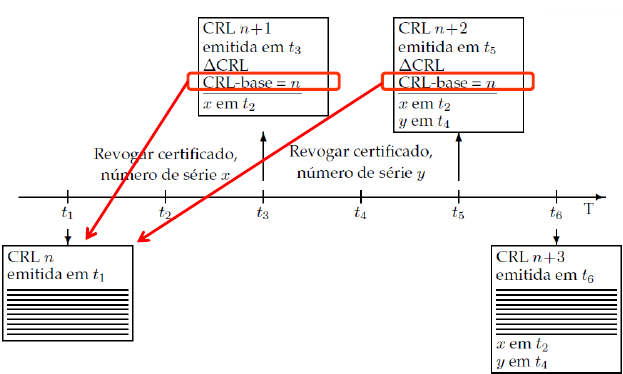
\includegraphics[scale=0.55]{17}
\end{center}

\pagebreak

\subsection{Online Certificate Status Protocol (OCSP)}

\begin{flushleft}
  \textbf{Protocolo baseado em HTTP para dar assert ao estado de um certificado}
  \begin{itemize}
    \item \textbf{Request} - Inclui o serial number do certificado;
    \item \textbf{Response} - Inclui se o certificado está revoked,
    é enviado pela CA e não possui validade;
    \item Uma verificação por certificado;
  \end{itemize}

  \vspace{2mm}

  \textbf{Requer menor largura de banda para clientes} -
  uma verificação por certificado em vez que fazer
  download de uma lista de certificados revogados (CRL);

  \vspace{2mm}

  \textbf{Involve maior largura de bannda para CAs} -
  uma verificação por certificado, problemas de privacidade
  uma vez que um CA saberá que um certificado está a ser usado;
  
  \vspace{2mm}

  \textbf{OOCSP stapling} - Inclui um timestamp recentemente assinado
  na resposta do servidor para dar assert à validade. Reduz a demora
  da verificação e carregamento no CA. Previne problemas de privacidade.
\end{flushleft}

\subsection{Distribuição de certificados de chaves públicas}

\begin{flushleft}
  \textbf{Transparente (integrado com sistemas ou aplicações)}
  \begin{itemize}
    \item Direcory systems, larga escala (ex: X.500 através de LDAP),
    organizacional (ex: Windows 2000 Active Directory), etc.;
    \item On-line: sem protocolos que usam certificados
    para autenticação peer (ex: protocolos de comunicação segura
    (TLS, IPSec, etc.), assinaturas digitais, dentro de MIME
    mail messages ou dentro de documentos);
  \end{itemize}

  \vspace{2mm}

  \textbf{Explicito (voluntáriamente ativado pelos users)}
  \begin{itemize}
    \item User faz request de um serviço para obter um certificado
    necessário (ex: pedido mandado por email, acesso a uma página HTTP pessoal).
  \end{itemize}
\end{flushleft}

\subsection{PKI (Public Key Infrastructure)}

\textbf{Infrastrutura para permitir um uso correto de chaves assimétricas e
de certificados de chave pública}.

\begin{flushleft}
  \textbf{Criação do par de chaves assimétricas para cada entidade que participa}.
  Politicas de participação, ploiticas de geração do par de chaves.

  \vspace{2mm}

  \textbf{Criação e distribuição de certificados de chaves públicas}.
  Politicas de participação, definição de atributos de certificados.

  \pagebreak

  \textbf{Definição e uso de certification chains (ou paths)}.
  Inserção numa hierarquia de certificação,
  certificação de outros CAs.

  \vspace{2mm}

  \textbf{Atualização, publicação e consulta de CRLs}.
  Politicas de revogação de certificados,
  serviços de distribuição de CRL, serviços OCSP.

  \vspace{2mm}

  \textbf{Usa estruturas de dados e protocolos permitindo inter-operabilidade
  entre componentes/serviços/pessoas}.
\end{flushleft}

\begin{center}
  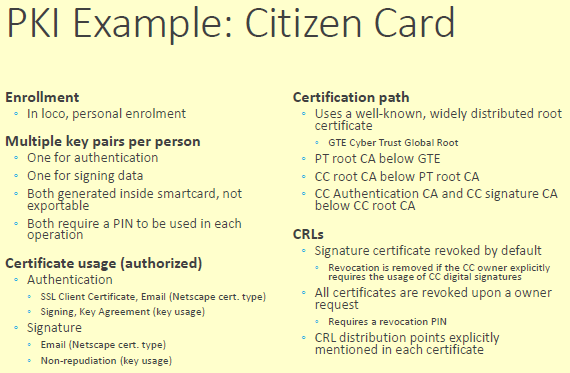
\includegraphics[scale=0.6]{18}
\end{center}

\subsection{Certificate Pinning}

\begin{flushleft}
  \textbf{Se um atacante tem acesso a uma Root confiavel, pode
  fingir ser qualquer entidade}. Manipula um CA confiavel
  em dar issue ao certificado (pouco provável).
  Injetar um CA costumizado na base de dados da vitima (mais provável).

  \vspace{2mm}

  \textbf{Certificate Pinning: adiciona a fingerprint do PubK (public key)
  ao \uline{código fonte}}. A fingerprint é uma hash (ex: SHA256).

  \vspace{2mm}

  \textbf{Validação do processo:} O certificado deve ser válido a regras locais,
  deve possuir uma chave pública com a dada fingerprint.
\end{flushleft}

\subsection{Certificate Transparency (RFC 6962)}

\begin{flushleft}
  \textbf{Problemas}
  \begin{itemize}
    \item CAs podem ser comprometidos (ex: DigiNotar) por atacantes,
    governo, etc.
    \item Comprometer é dificil de detetar. Resulta na mudança de
    suposições associadas com o comportamento do CA.
    O proprietário saberá sozinho.
  \end{itemize}

  \vspace{2mm}

  \textbf{Definição: um sistema global que regista todas as informações sobre
  certificados públicos criados}
  \begin{itemize}
    \item Garante que apenas um certificado tem as roots corretas;
    \item Guarda a chain de certificados inteira para cada certificado;
    \item Apresenta esta informação para auditoria (organizações
    ou ad-hoc por end users);
  \end{itemize}
\end{flushleft}

\end{document}